% !TEX root = ../main.tex

% 中英标题：\chapter{中文标题}[英文标题]

\chapter{目前已完成的主要研究工作及结果}
\section{数据集的获取及预处理}
\subsection{数据集的获取}
为实现和评估本课题提出的多模态蛋白质功能预测模型，我们从多个权威公共数据库中获取了蛋白质的序列、结构和功能注释等相关数据。数据覆盖范围广泛、注释质量可靠，能够支持有监督学习与零样本预测的多任务建模。

蛋白质序列数据来源于 UniProtKB/Swiss-Prot 数据库\cite{uniprot2023uniprot},蛋白质三维结构数据由 AlphaFold Protein Structure Database \cite{varadi2022alphafold}提供,功能注释（GO术语） 从 Gene Ontology Annotation (GOA) 数据库\cite{huntley2015goa}中获取。为构建统一的数据集，我们对三类数据进行了严格的样本级对齐：仅保留同时具备序列、结构和高置信度 GO 注释的蛋白质样本,移除重复序列以及长度超过 10,000 个氨基酸的序列。

数据集划分：监督学习数据集遵循 ProteInfer\cite{sanderson2023proteinfer}的随机拆分方案，将数据划分为训练集（80\%）、验证集（10\%）和测试集（10\%）,该数据集基于 2019年7月1日发布的 GO 注释版本构建。为评估模型对未见过的蛋白质和新功能的预测能力，我们构建了一个专门的零样本测试集。该数据集包含序列在 2019年7月至 2024年5月期间新添加到 Swiss-Prot 数据库的蛋白质序列，GO术语为词汇外（out-of-vocabulary）术语，即那些在 2019年7月1日之后才首次在 GO 本体中被定义的功能，注释来源于 2024年6月17日发布的 GO 注释版本。

最终整理所得的多模态蛋白质功能预测数据集，涵盖多个物种与结构类型，具备序列、结构、GO功能注释及文本描述信息，能够全面支撑本课题所提出模型的训练（监督学习）与测试（监督学习、零样本预测）需求。数据集的详细统计信息如表2-1所示。
\begin{table}[h!]
\centering
\caption{蛋白质数据集统计信息}
\begin{tabular}{@{}ccccccc@{}}

\toprule
划分方式 & 生物过程（BPO） & 细胞成分（CCO） & 分子功能（MFO） & 全部 \\
\midrule
GO-Rand-Train & 38,185 & 34,313 & 25,405 & 45,803 \\
GO-Rand-Val & 4,773 & 4,289 & 3,176 & 5,725 \\
GO-Rand-Test & 4,773 & 4,289 & 3,175 & 5,726 \\
GO-Zero-Shot &2067  &1988  &1326  & 2445 \\
\bottomrule
\end{tabular}
\end{table}
\subsection{数据预处理}
本课题对收集并对齐后的蛋白质数据进行了以下预处理操作：序列信息统一采用 UniProt 中的标准 FASTA 格式,使用 ESM-2 蛋白质语言模型对每条蛋白质序列进行特征提取，生成氨基酸级别的语义向量表示；结构信息解析 AlphaFold 数据库提供的蛋白质三维结构文件（PDB格式），提取每个氨基酸残基的 Cα 原子坐标，基于坐标计算并构建残基接触图（Contact Map），在接触图基础上添加三类结构边关系，构建用于异构图建模的初始图结构。序列边 (Sequence Edge): 连接相邻残基；K近邻边 (K-Nearest Neighbors Edge): 连接空间距离最近的 K 个残基；空间半径边 (Spatial Radius Edge): 连接空间距离小于给定半径阈值的残基对。

然后本课题还需要对 GO 标签进行预处理， GOA 数据库中收录了多种来源的 GO 标签，为了保证GO 标签的真实性，本课题仅选择了专家手工收集和实验得到的GO 标签，即保留了来源为 EXP、IDA、IPI、IMP、IGI、IEP、HTP、HAD、HMP、HGI、HEP、
IBA、IBD、IKR、IRD 的GO 标签\cite{barrell2009goa}。由于 GO 标签在基因本体库[12]的对应分支中构成一张有向无环图，且具有父子关系，如图 2-1 所示。
\begin{figure}[h]
\centering
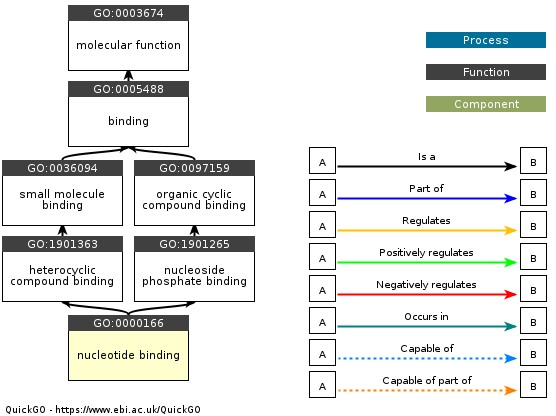
\includegraphics[width = 1\textwidth]{figures/1.jpg}
\caption{GO树状结构示例\cite{binns2009quickgo}}
\label{fig:go}
\end{figure}

根据真实路径规则，子节点具有父节点的功能，意味着一个蛋白质若具有某一 GO标签，那么它同时具有该 GO 标签的所有父节点。因此，本课题在实验中记录了GO 之间的“is a”和“part of”关系，以此构建了 GO 的树形结构，然后以每一个蛋白质的当
前的GO 标签为依据向上传播，将途径的 GO 标签都加入到该蛋白质的标签集合中，直到其GO 标签集合不再增加。预处理后每个分支上的标签数量如表 2-2 所示。
\begin{table}[h!]
\centering
\caption{GO 标签数量统计}
\label{tab:go_term_counts}
\begin{tabular}{lccc}
\toprule
基因本体分支 & 生物过程（BPO） & 分子功能（MFO） & 细胞成分（CCO） \\
\midrule
有监督预测GO数量 & 19,450 & 6,095 & 2,515 \\
零样本预测GO数量 & 497 & 286 & 203 \\
\bottomrule
\end{tabular}
\end{table}

\section{基于多模态预训练的蛋白质功能预测模型}
为充分挖掘蛋白质序列、结构与功能语义之间的关联信息，本课题提出了一种基于多模态预训练的蛋白质功能预测模型，整体架构如图2-2所示。
\begin{figure}[h]
\centering
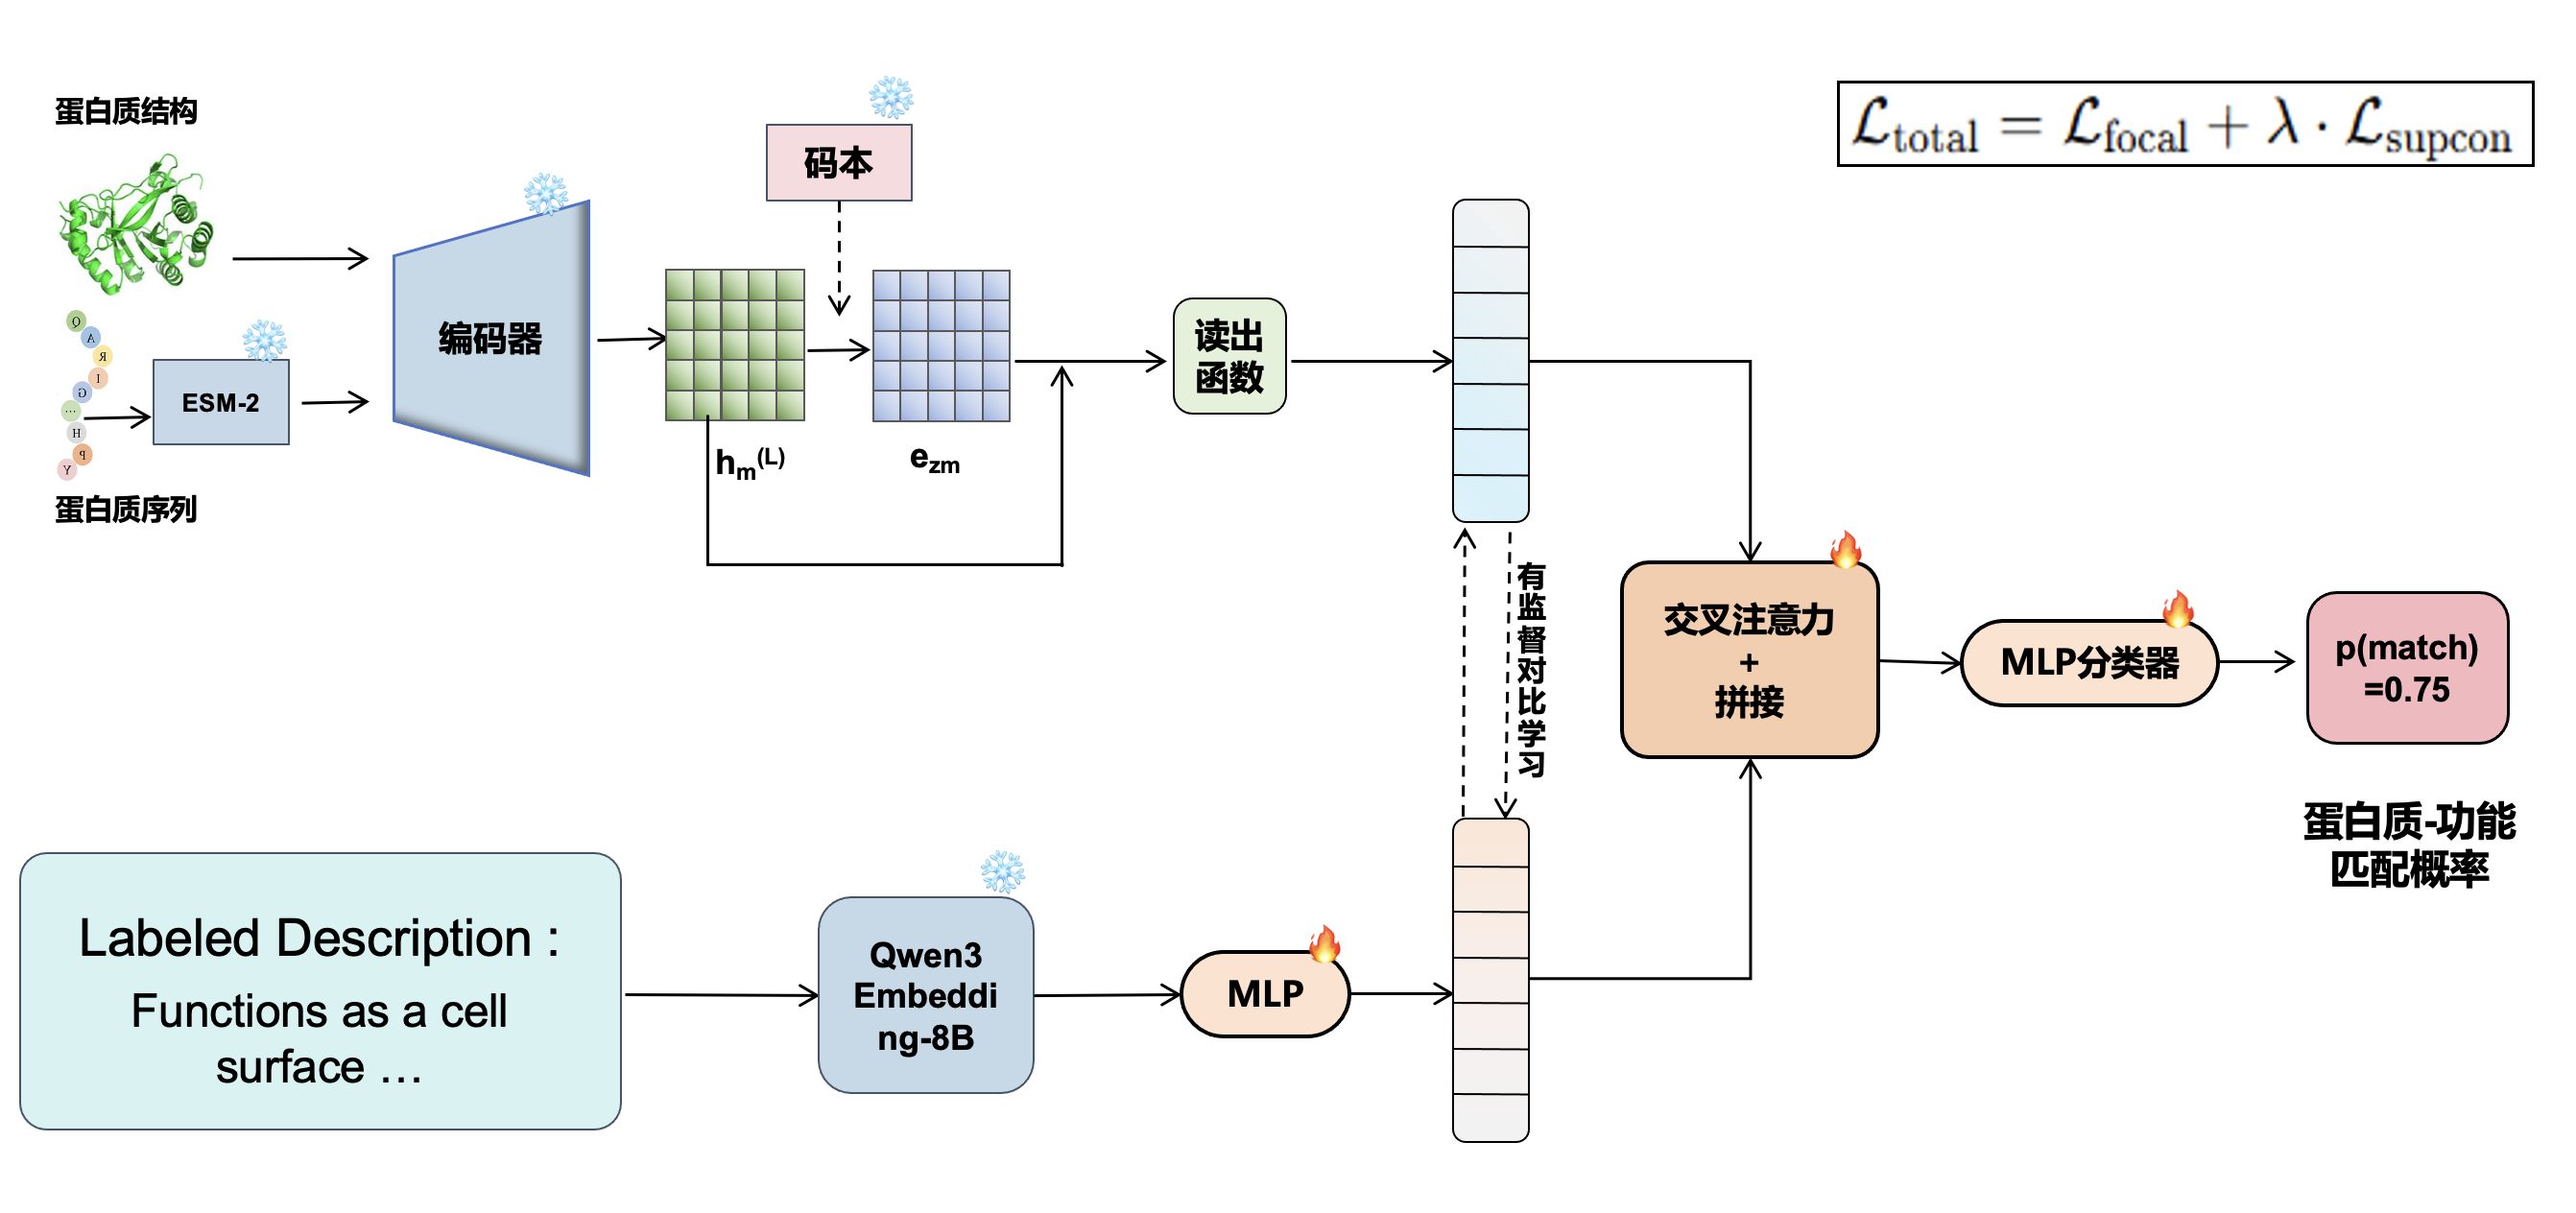
\includegraphics[width = 1\textwidth]{figures/predict.png}
\caption{基于多模态预训练的蛋白质功能预测模型架构}
\label{fig:predict}
\end{figure}

在多模态编码器设计中，模型融合来自序列和结构两类异质信息。具体而言，序列信息通过预训练语言模型 ESM-2 提取，获取氨基酸序列的深层语义表示；结构信息首先构建接触图，引入序列边、K近邻边与空间半径边三类拓扑关系，进一步构建异构图结构，并借助异构图神经网络（HGNN）实现蛋白质多模态表征的统一编码。

为有效引入功能语义信息，采用文本嵌入模型Qwen3-Embedding对 Gene Ontology (GO) 功能标签的文本描述进行语义嵌入，获得具有上下文感知能力的标签表示。该语义表示不仅用于有监督分类任务，也作为对比学习的目标，增强蛋白质表示与功能语义之间的对齐能力。

训练流程采用分阶段设计。首先在多模态预训练阶段，通过掩码恢复与特征重建任务强化结构与序列表示之间的耦合一致性，随后进入有监督的多任务训练阶段，主任务使用基于 Focal Loss 的分类器对 GO 注释进行预测，以强化模型对长尾标签的识别能力；辅助任务以对比学习作为分支，进一步提升模型在零样本功能预测场景下的泛化能力与语义判别能力。本节将围绕上述模型各模块的关键实现方法与训练机制展开详细介绍。

\subsection{蛋白质序列和结构的预训练特征提取}

本课题提出了一种结合序列语义、结构建模与图掩码重建的多模态预训练机制。该机制将 ESM-2 生成的氨基酸级别表示作为节点初始化特征，并构建异构图进行图神经网络传播，进一步通过蛋白质码本进行结构感知的离散建模，整体结构如图~\ref{fig:pretrain} 所示。

\begin{figure}[h]
\centering
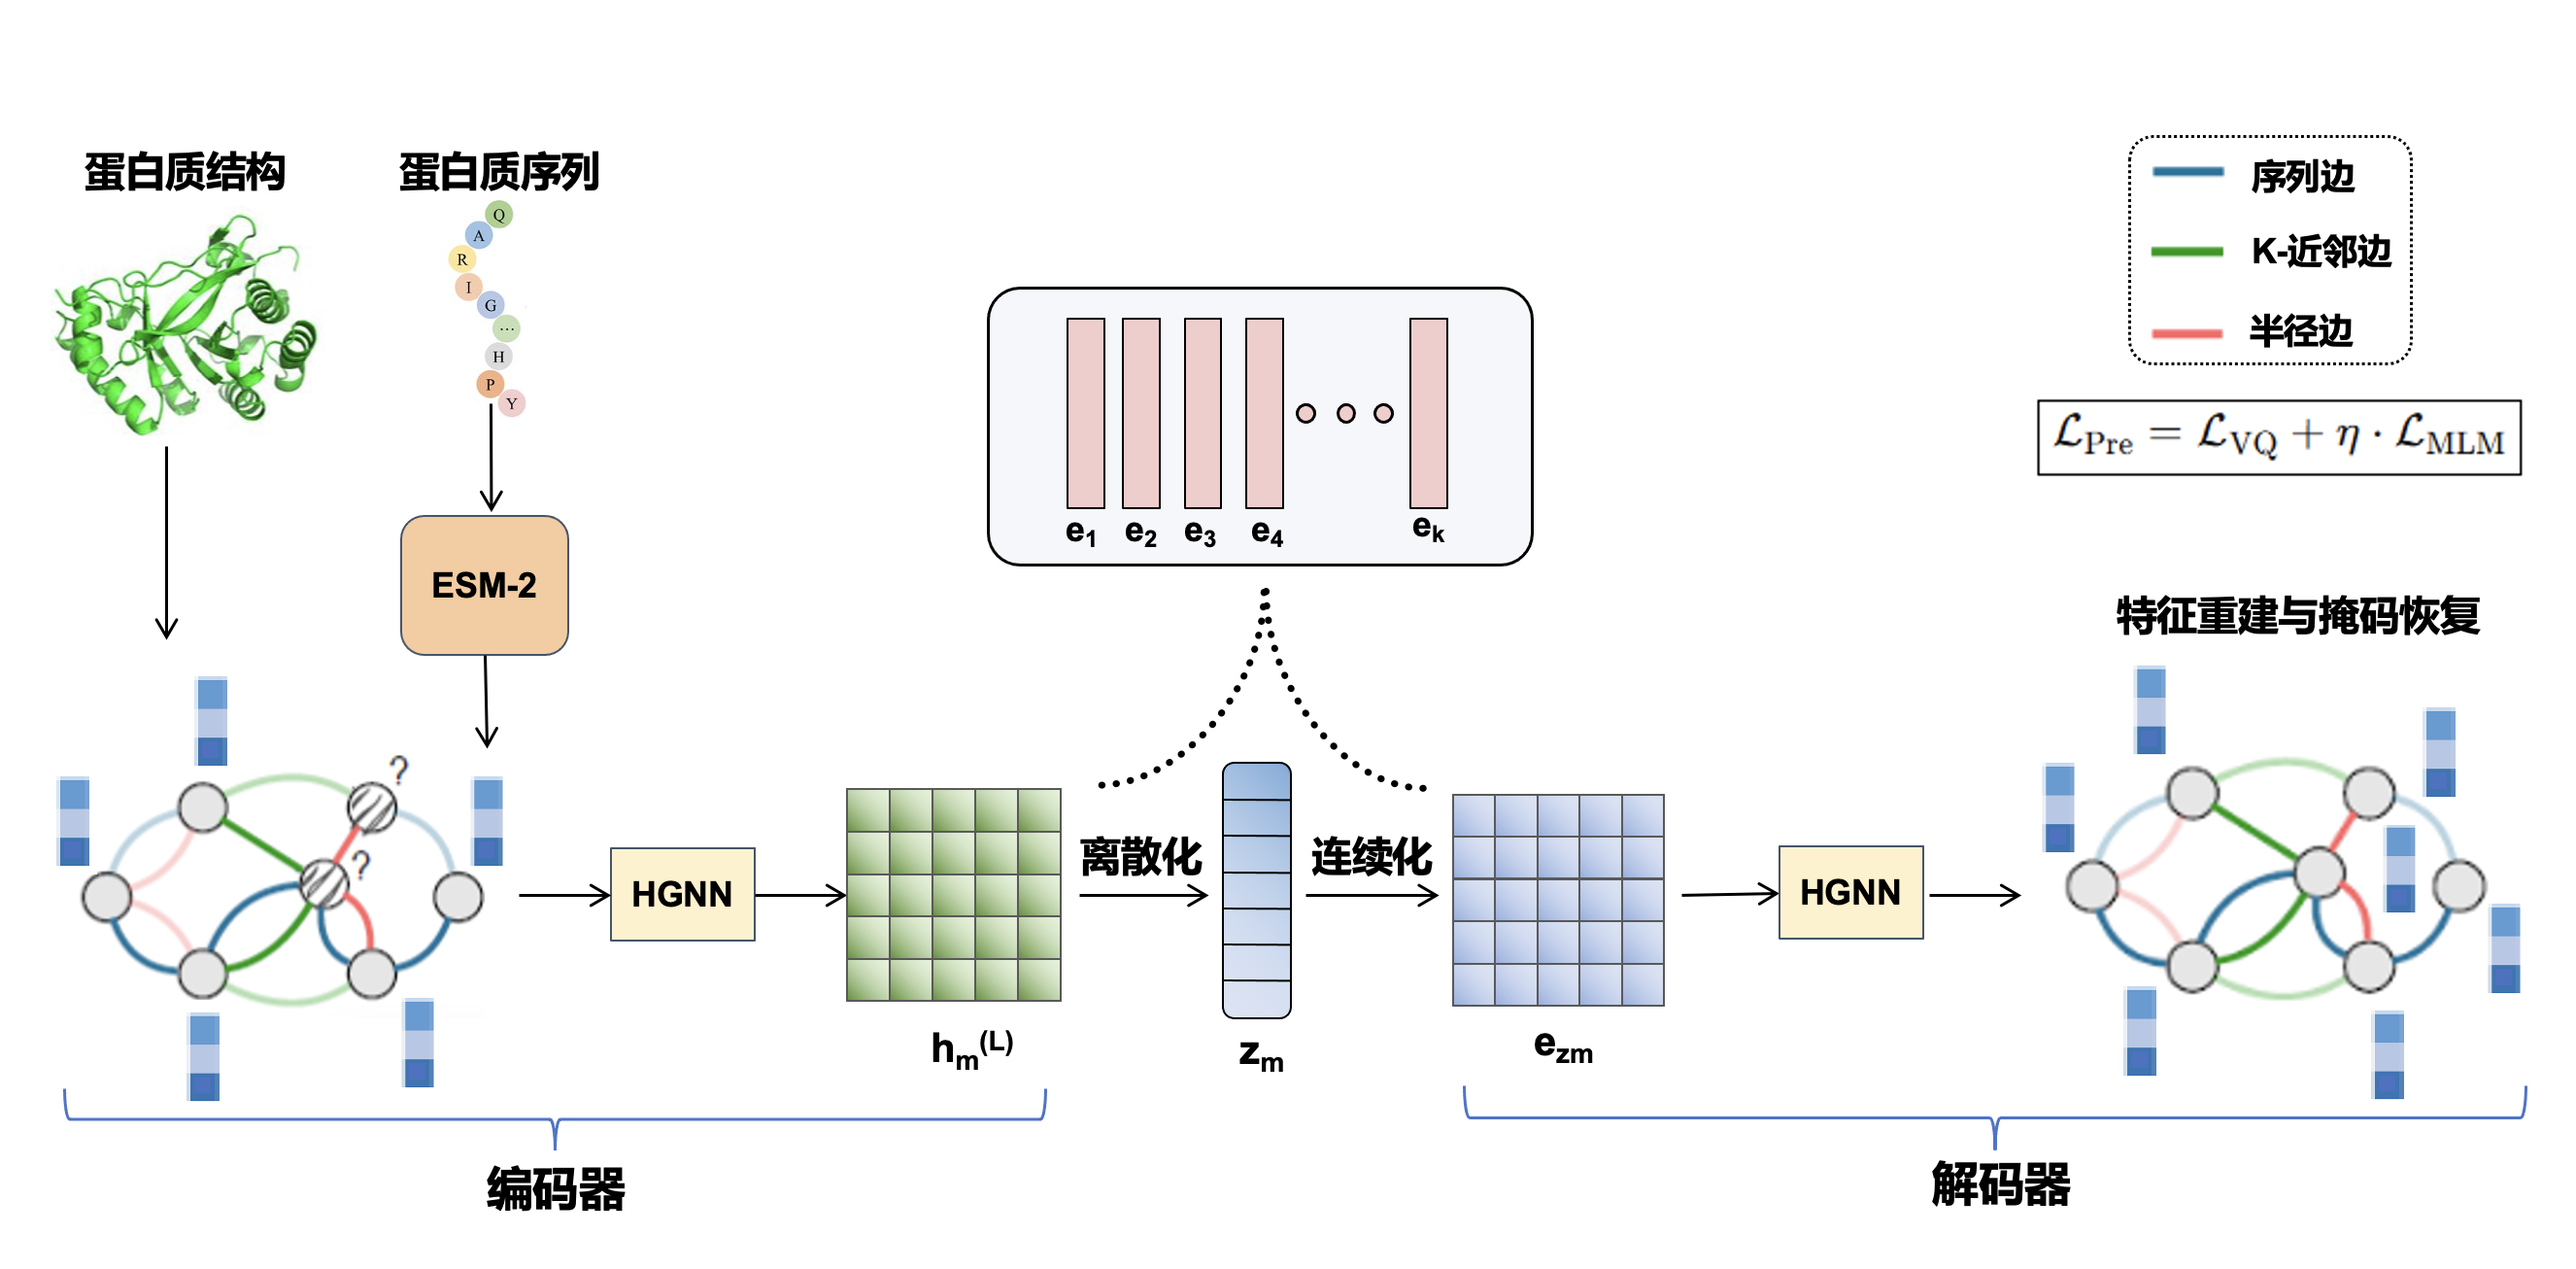
\includegraphics[width = 1\textwidth]{figures/pretrain.png}
\caption{蛋白质序列和结构的预训练架构}
\label{fig:pretrain}
\end{figure}

我们首先使用 ESM-2 模型对蛋白质序列进行编码，获得每个残基的上下文语义表示 $\{x_1, x_2, \ldots, x_L\}$，其中 $L$ 为蛋白质的氨基酸序列长度，$x_i \in \mathbb{R}^{1280}$ 表示第 $i$ 个残基的上下文嵌入。在结构方面，利用 AlphaFold2预测的蛋白质三维结构，提取 C$_\alpha$ 原子坐标，构建包含以下三种边类型的残基异构图：

\begin{itemize}
  \item 序列边：连接序列中相邻残基，捕捉一级结构信息；
  \item K-近邻边：连接空间上欧氏距离最近的 $k=10$ 个残基；
  \item 半径边：连接欧氏距离小于 $10\text{\AA}$ 的残基对。
\end{itemize}

每个图节点以其对应的ESM-2残基嵌入作为初始特征输入到异构图神经网络（HGNN）编码器中。HGNN 能够处理含有多种边类型的异构图结构，在每一层中融合不同边类型带来的拓扑信息和语义特征。考虑 $L$ 层 HGNN 编码器，第 $l$ 层的传播公式定义如下：
\begin{equation}
\mathbf{h}_m^{(l)} = \text{BN}\left( 
\text{ReLU} \left( 
\mathbf{W}_h^{(l)} \cdot \sum_{r \in \mathcal{R}} \mathbf{W}_r^{(l)} \cdot \sum_{v_n \in \mathcal{N}_r(m)} \mathbf{h}_n^{(l-1)} 
\right) 
\right), \quad \text{for } 1 \leq l \leq L
\end{equation}
其中，$\mathcal{R}$ 表示边类型集合，$\mathcal{N}_r(m)$ 表示节点 $v_m$ 在边类型 $r$ 下的邻居集合，$\mathbf{W}_r^{(l)}$ 和 $\mathbf{W}_h^{(l)}$ 分别为边类型转换矩阵与整体融合线性变换矩阵，BN 表示 Batch Normalization，ReLU 为激活函数。通过多层 HGNN 聚合后，得到每个残基的最终嵌入表示 $\mathbf{h}_i^{(L)}$，该表示融合了局部空间环境、拓扑上下文与序列语义等多模态信息。为了提升模型的泛化性建模蛋白质的离散结构向量，我们引入 VQ-VAE \cite{yan2021videogpt}框架对残基表示进行离散化，构建可学习的码本 $\mathcal{C} = \{e_1, e_2, \ldots, e_K\}$，并将每个 $h_i^{(L)}$ 映射至最近的码本向量 $z_i$：
\begin{equation}
z_i = \arg\min_{e_j \in \mathcal{C}} \| h_i^{(L)} - e_j \|_2
\end{equation}

离散化后的向量 $z_i$ 再进行连续化处理后输入到对称结构的 HGNN 解码器中，用于特征重建。为了进一步增强模型对节点语义的感知能力，我们在图神经网络输入层进行掩码建模。具体做法是：随机选择部分残基节点（15\%）进行特征掩码，用特殊 token 替代原始嵌入；模型需在整图上下文信息基础上重建被掩码节点的原始特征 $x_i$。

最终的预训练目标为联合优化离散建模损失 $\mathcal{L}_{\text{VQ}}$ 与图掩码重建损失 $\mathcal{L}_{\text{MLM}}$。$\mathcal{L}_{\text{VQ}}$ 源于 VQ-VAE 框架，包含三部分组成：
\begin{equation}
\mathcal{L}_{\text{VQ}} = 
\underbrace{\sum_i \| x_i - \hat{x}_i \|_2^2}_{\text{重构损失}} + 
\underbrace{\sum_i \| \text{sg}[h_i^{(L)}] - z_i \|_2^2}_{\text{码本更新损失}} + 
\underbrace{\beta \sum_i \| h_i^{(L)} - \text{sg}[z_i] \|_2^2}_{\text{编码器回传损失}}
\end{equation}
其中，$\text{sg}[\cdot]$ 表示 stop-gradient 操作，$\hat{x}_i$ 为解码器重构得到的特征，$\beta$ 为调节项，控制编码器更新强度。

$\mathcal{L}_{\text{MLM}}$ 表示掩码节点特征的重建损失，用于学习结构图中局部语义之间的依赖关系。定义如下：
\begin{equation}
\mathcal{L}_{\text{MLM}} = \sum_{i \in \mathcal{M}} \| \hat{x}_i - x_i \|_2^2
\end{equation}
其中，$\mathcal{M}$ 表示掩码位置集合，$\hat{x}_i$ 为模型对掩码位置 $i$ 的重建特征，$x_i$ 为其真实特征。
整体损失函数定义为：
\begin{equation}
\mathcal{L}_{\text{Pre}} = \mathcal{L}_{\text{VQ}} + \eta \cdot \mathcal{L}_{\text{MLM}}
\end{equation}
其中，$\eta$ 为平衡系数，实验中设置为 0.5。该预训练机制使模型在保留语义上下文的同时具备结构感知能力，为下游的功能预测、语义对齐与零样本推理提供高质量的初始嵌入表示。


\subsection{GO标签的语义嵌入与蛋白质表示建模}
为实现蛋白质与功能标签之间的语义对齐与零样本功能预测能力，本课题设计了面向 Gene Ontology (GO) 标签的语义建模机制与蛋白质功能表示生成模块。GO 是结构化的生物本体体系，其术语以自然语言定义，用于描述蛋白质的分子功能（Molecular Function）、生物过程（Biological Process）及细胞成分（Cellular Component）等。传统方法常将 GO 标签视作离散类别索引，忽略其语言语义与本体结构信息，难以捕捉标签间的潜在语义关系，也无法推广到未标注类别。

为克服上述局限，本课题引入文本嵌入模型对 GO 标签文本进行嵌入建模，将自然语言定义编码为连续向量表示。具体而言，对于每个 GO 标签，我们使用其定义描述文本作为输入，例如：

\textit{protein kinase activity: Catalysis of the transfer of a phosphate group to a protein substrate.}

将该描述输入 Qwen3-Embedding-8B 模型后，提取其句向量作为语义嵌入，记为 $\mathbf{E}_{\text{GO}}^{\text{raw}} \in \mathbb{R}^{4096}$。为将该高维语义表示投影到与蛋白质嵌入一致的空间中，我们引入多层感知机（MLP）对其进行线性变换，得到最终的 GO 向量表示：
\begin{equation}
\mathbf{E}_{\text{GO}} = \text{MLP}_{\text{GO}}(\mathbf{E}_{\text{GO}}^{\text{raw}}) \in \mathbb{R}^{d}
\end{equation}
其中，$d=2304$ 为模型统一的语义表示维度。该向量不仅保留了 GO 标签的语言语义，还与蛋白质嵌入向量共享空间，为语义相似度计算与功能分类提供基础。之所以选择文本嵌入模型而非生物医学特定模型BioGPT，是因为实验验证文本嵌入模型作为标签编码器时性能更好。我们推测这可能是因为Embedding模型的高质量句子嵌入，而像BioGPT这样的模型是通过平均token级嵌入来提取句子嵌入的。

蛋白质表示则由多模态特征提取得到。我们首先使用 ESM-2 模型对蛋白质序列进行编码，获得每个残基的上下文语义表示 $\mathbf{x}_m \in \mathbb{R}^{1280}$。该表示作为节点特征，与蛋白质结构图联合输入至图神经编码器，得到融合结构语义的残基嵌入 $\mathbf{h}_m^{(L)} \in \mathbb{R}^{d}$。

随后，利用已训练好的蛋白质码本 $\mathcal{C} = \{e_1, e_2, \ldots, e_K\} \subset \mathbb{R}^{1024}$ 对每个残基的蛋白质表示进行离散编码与向量查找，得到其对应的码本嵌入 $\mathbf{e}_{z_m} \in \mathbb{R}^{1024}$。将其与图神经输出 $\mathbf{h}_m^{(L)}$ 进行拼接，得到残基级多模态表示：
\begin{equation}
\mathbf{u}_m = \mathbf{e}_{z_m} \, \| \, \mathbf{h}_m^{(L)} \in \mathbb{R}^{d}
\end{equation}
其中 ，$\|$ 表示向量拼接操作。为了将残基级表示整合为蛋白质级别的全局表示，定义读出函数 $\text{READOUT}(\cdot)$ 对所有残基表示进行平均池化：
\begin{equation}
\mathbf{H}_{\text{P}} = \text{READOUT} \left( \left\{ \mathbf{u}_m \right\}_{m=1}^{L} \right) = \frac{1}{L} \sum_{m=1}^{L} \mathbf{u}_m \in \mathbb{R}^{d}
\end{equation}
其中， $L$ 表示蛋白质的残基数量。最终，蛋白质表示 $\mathbf{H}_{\text{P}}$ 与 GO文本嵌入 $\mathbf{E}_{\text{GO}}$ 共存于统一的语义嵌入空间中，便于进行相似度匹配、语义分类等下游任务。



\subsection{多任务学习框架与功能预测机制}

为了同时提升模型在有监督GO功能分类与零样本功能预测场景下的表现，本课题设计了一种基于统一表示空间的多任务学习框架。该框架以蛋白质的多模态表示 $\mathbf{H}_{\text{P}} \in \mathbb{R}^d$ 与 GO 标签的语义嵌入表示 $\mathbf{E}_{\text{GO}} \in \mathbb{R}^d$ 为基础，对每一个蛋白质–GO标签对构建融合表示，借助交叉注意力机制实现语义交互，并通过拼接形成对偶表示，输入多层感知机（MLP）进行预测，从而判断某一蛋白质是否具有该GO功能。同时，辅以语义匹配的对比学习任务，以提升模型的泛化能力与标签感知能力。

在特征融合阶段，采用交叉注意力机制\cite{hou2019cross}以蛋白质表示作为查询（Query），GO标签表示作为键值对（Key/Value），提取语义交互信息。其基本计算形式为：
\begin{equation}
\text{Attention}(\mathbf{Q}, \mathbf{K}, \mathbf{V}) = \text{softmax}\left( \frac{\mathbf{Q} \mathbf{K}^\top}{\sqrt{d}} \right)\mathbf{V}
\end{equation}
其中，
\begin{equation}
\mathbf{Q} = \mathbf{W}_Q \mathbf{H}_{\text{P}}, \quad \mathbf{K} = \mathbf{W}_K \mathbf{E}_{\text{GO}}, \quad \mathbf{V} = \mathbf{W}_V \mathbf{E}_{\text{GO}}
\end{equation}
$\mathbf{W}_Q, \mathbf{W}_K, \mathbf{W}_V \in \mathbb{R}^{d \times d_a}$ 为可学习的线性映射，$d_a$ 为注意力维度，本课题采用多头交叉注意力机制，将多个子空间中学到的注意力结果拼接后映射为原始维度，最终获得融合GO语义的蛋白质交互表示 $\mathbf{F}_{\text{attn}} \in \mathbb{R}^d$。

最终将蛋白质表示与交叉注意力输出拼接，构成蛋白质–GO对的联合表示：
\begin{equation}
\mathbf{F}_{\text{joint}} = \mathbf{H}_{\text{P}} \, \| \, \mathbf{F}_{\text{attn}} \in \mathbb{R}^{2d}
\end{equation}

该联合表示输入至MLP分类器 $\text{MLP}_{\text{cls}}$，输出该蛋白质–GO对的二分类概率：
\begin{equation}
\hat{y}_{(P, GO)} = \text{MLP}_{\text{cls}}(\mathbf{F}_{\text{joint}}) \in [0, 1]
\end{equation}
其中 ，$\hat{y}_{(P, GO)}$ 表示预测该蛋白质是否具有该GO功能。

考虑到GO标签之间存在严重的长尾分布，频繁标签与低频标签之间样本量差异较大，直接使用二分类交叉熵可能导致模型偏向主频标签，因此引入Focal Loss以提升对困难负样本与低频类别的学习能力，损失函数如下：
\begin{equation}
\mathcal{L}_{\text{focal}} = -\alpha_t (1 - p_t)^\gamma \log(p_t)
\end{equation}
其中 ，$p_t = \hat{y}_{(P, GO)}$ 为预测概率，$\alpha_t$ 为调节正负样本重要性的因子，$\gamma$ 为调节困难样本关注度的聚焦因子。

为进一步提升模型对未见GO标签的泛化能力，辅助任务采用有监督对比学习（Supervised Contrastive Learning）约束蛋白质表示与功能标签语义嵌入之间的一致性。具体地，模型在一个批次内将同一蛋白质对应的所有真实GO标签嵌入视为正样本，其他非关联标签嵌入作为负样本，推动模型学习“蛋白质–功能语义”空间中更加紧密的对齐结构。其损失函数定义如下：
\begin{equation}
\mathcal{L}_{\mathrm{supcon}} = \frac{-1}{|P(i)|} \sum_{p \in P(i)} \log \frac{
    \exp\left(\mathrm{sim}\big(\mathbf{H}_{\mathrm{P}}^{(i)}, \mathbf{E}_{\mathrm{GO}}^{(p)}\big) / \tau\right)
}{
    \sum_{a \in A(i)} \exp\left(\mathrm{sim}\big(\mathbf{H}_{\mathrm{P}}^{(i)}, \mathbf{E}_{\mathrm{GO}}^{(a)}\big) / \tau\right)
}
\end{equation}

其中，\( \mathbf{H}_{\mathrm{P}}^{(i)} \) 表示第 \(i\) 个蛋白质的嵌入，\( P(i) \) 表示该蛋白质对应的正样本GO标签索引集合，\( A(i) \) 表示同批次中除自身外的所有标签索引集合（包含正负样本），\(\mathrm{sim}(\cdot,\cdot)\) 表示余弦相似度，\(\tau\) 为温度系数。

该损失鼓励模型将蛋白质表示与其真实GO标签嵌入在语义空间中拉近距离，同时推开非关联标签嵌入，从而显著提升模型对未见功能标签的预测泛化能力。最终，该多任务学习框架通过共享编码器进行联合优化，其总损失函数为：
\begin{equation}
\mathcal{L}_{\text{total}} = \mathcal{L}_{\text{focal}} + \lambda \cdot \mathcal{L}_{\text{supcon}}
\end{equation}
其中， $\lambda$ 为权重超参数，用于平衡二分类精度与语义对齐之间的贡献，实验中设置为 $\lambda=0.3$。

该多任务学习策略实现了蛋白质与功能标签之间的细粒度匹配，充分发挥了分类器在高质量标注下的判别能力与语义对比机制在未见标签下的迁移能力，提升了模型在不同数据分布与标签集合下的适应性与泛化能力，适用于多物种、多场景下的蛋白质功能注释任务。



\section{评价指标和实验分析}
本课题设计了一种融合蛋白质序列、结构与功能语义信息的模型，适用于蛋白质的功能预测任务，能够同时支持有监督分类与零样本语义匹配。为了验证所提模型在不同任务场景下的性能与泛化能力，本课题在多个真实数据集上进行了系统的对比实验与消融实验，并采用多种主流评价指标对模型效果进行评估,全面反映模型的有效性与优势。

\subsection{评价指标}
本课题属于蛋白质功能的多标签预测任务。由于标签分布存在极度不均衡，存在大量长尾标签与低频GO功能，传统的准确率或AUC-ROC指标在衡量模型整体性能方面存在局限，难以全面反映模型在少标签预测与语义泛化方面的效果，特别是难以公正评估模型在大量低频标签上的性能。为此，本课题采用两种基于精确率-召回率曲线下面积（Area Under the Precision-Recall Curve, AUPRC）且更适合多标签不平衡分类场景的评估指标：宏平均平均精度（Macro-mAP）和微平均平均精度（Micro-mAP）。

Macro-mAP的计算过程是：首先为数据集中的每个标签（GO term）独立计算其精确率-召回率曲线下的面积（即该标签的Average Precision, AP），然后对所有标签的AP值进行简单算术平均。其公式表示为：
\begin{equation}
\text{Macro-mAP} = \frac{1}{|L|} \sum_{l=1}^{|L|} AP_l
\end{equation}
其中，$L$是标签集合，$|L|$是标签总数，$AP_l$是第$l$个标签的平均精度。

Micro-mAP的计算过程是：首先将所有样本在所有标签上的预测结果汇总，形成一个全局的混淆矩阵，然后基于这个全局混淆矩阵计算单一的精确率-召回率曲线，并计算该曲线下的面积。其公式等效于：
\begin{align}
\text{Precision}_{\text{micro}} &= \frac{\sum_{l=1}^{|L|} TP_l}{\sum_{l=1}^{|L|} (TP_l + FP_l)} \\
\text{Recall}_{\text{micro}} &= \frac{\sum_{l=1}^{|L|} TP_l}{\sum_{l=1}^{|L|} (TP_l + FN_l)} \\
\text{Micro-mAP} &= \int_{0}^{1} \text{Precision}_{\text{micro}} \, d(\text{Recall}_{\text{micro}})
\end{align}
其中，$TP_l$, $FP_l$, $FN_l$分别表示在标签$l$上的真阳性、假阳性和假阴性数量。

在指标选择方面：Macro-mAP为每个标签赋予同等权重，无论其出现的频率高低。其计算结果不受标签分布偏差的影响，能够更公平地评估模型在大量低频、长尾GO标签上的预测能力（98\%的GO术语出现在不超过1\%的序列中），这对于本课题关注语义泛化到罕见功能的需求至关重要。因此，本课题选用Macro-mAP作为模型选择的主要依据。另一方面，Micro-mAP的计算结果受标签分布的影响，高频标签对最终得分的贡献更大，这在需要优化对高频出现结果的预测时具有参考价值。

相比依赖于特定决策阈值的指标（如$F_{\text{max}}$或F1分数），Macro-mAP和Micro-mAP通过汇总模型在所有可能预测阈值下的性能，提供了更全面、更鲁棒的性能评估。它们能更好地反映模型在高度不平衡的多标签分类任务中的整体表现。

综上，Macro-mAP值越高、Micro-mAP值越高，表明模型在预测准确性和标签覆盖能力上的表现越优，尤其适合评估本课题所提出的多模态模型在长尾标签、零样本类别上的性能优势。后续实验部分将基于这两个指标对模型进行定量评估与对比分析。

\subsection{对比实验与结果分析}
本课题进行了系统的性能评估，涵盖监督学习和零样本学习两种场景。在监督学习场景下，与蛋白质功能预测领域的代表性方法进行对比，包括基于序列相似性的传统方法BLAST\cite{altschul1990basic}、深度学习模型ProteInfer\cite{sanderson2023proteinfer}以及支持零样本学习的新型架构ProtNote\cite{char2025protnote}。如表2-3所示，本模型在监督学习场景展现出差异化优势：在CCO（细胞成分）本体上以\textbf{0.652}的Macro-mAP优于ProtNote(0.587)和ProteInfer(0.637)，相对提升达11.1\%；在MFO（分子功能）本体上以0.794接近最优方法ProteInfer(0.805)；在BPO（生物过程）本体上(0.565)与最优方法存在差距。这种跨本体性能差异与不同本体的数据特性相关：MFO本体受益于蛋白质结构特征的加入，CCO本体的优异表现证明多模态融合能有效解决细胞定位预测的挑战，BPO本体的性能不佳可能受限于多模态信息引入了噪声。

\begin{table}[h]
\centering
\caption{监督学习场景下的Macro-mAP指标}
\begin{tabular}{lccc}
\hline
Methods & 生物过程（BPO） & 分子功能（MFO） & 细胞成分（CCO） \\
\hline
BLAST & 0.454 & 0.729 & 0.543 \\
ProteInfer & \textbf{0.587} & \textbf{0.805} & 0.637 \\
ProtNote & 0.568 & 0.707 & 0.587 \\
Mymodel & 0.565 & 0.794 & \textbf{0.652} \\
\hline
\end{tabular}
\end{table}

\begin{table}[h]
\centering
\caption{监督学习场景下的Micro-mAP指标}
\begin{tabular}{lccc}
\hline
Methods & 生物过程（BPO） & 分子功能（MFO） & 细胞成分（CCO） \\
\hline
BLAST & 0.744 & 0.912 & 0.763 \\
ProteInfer & 0.874 & 0.964 & 0.892 \\
ProtNote & 0.878 & \textbf{0.966} & 0.896 \\
Mymodel & \textbf{0.885} & 0.965 & \textbf{0.905} \\
\hline
\end{tabular}
\end{table}

针对新兴蛋白质功能的预测需求，本课题遵循ProtNote\cite{char2025protnote}提出的基准测试方法：对每个未见过的功能，首先使用文本嵌入模型将其功能描述转化为向量；其次通过余弦相似度，在训练集中找到与该描述最接近的已知功能；最后使用ProteInfer计算该已知功能的概率。我们在零样本场景下与文本增强基线进行对比，包括生物医学语言模型BioGPT\cite{luo2022biogpt}、多语言文本嵌入模型E5\cite{wang2024multilingual}、大语言文本嵌入模型Qwen3-Embedding\cite{qwen3embedding}以及当前最先进的零样本框架ProtNote\cite{char2025protnote}。如表2-4所示，本模型在零样本场景实现全面领先：在BPO(0.167)、MFO(0.393)、CCO(0.154)三个本体上均超越ProtNote，相对提升分别为13.6\%、6.8\%和10.8\%，体现了本模型在保持本体监督学习优势的同时，在零样本场景获得全面提升。

\begin{table}[h]
\centering
\caption{零样本学习场景下的Macro-mAP指标}
\begin{tabular}{lccc}
\hline
Methods & 生物过程（BPO） & 分子功能（MFO） & 细胞成分（CCO） \\
\hline
BioGPT & 0.083 & 0.194 & 0.107 \\
E5 & 0.112 & 0.255 & 0.068 \\
Qwen3-Embedding & 0.128 & 0.284 & 0.097 \\
ProtNote & 0.147 & 0.368 & 0.139 \\
Mymodel & \textbf{0.167} & \textbf{0.393} & \textbf{0.154} \\
\hline
\end{tabular}
\end{table}

\begin{table}[h]
\centering
\caption{零样本学习场景下的Micro-mAP指标}
\begin{tabular}{lccc}
\hline
Methods & 生物过程（BPO） & 分子功能（MFO） & 细胞成分（CCO） \\
\hline
BioGPT & 0.185 & 0.274 & 0.142 \\
E5 & 0.226 & 0.321 & 0.158 \\
Qwen3-Embedding & 0.248 & 0.358 & 0.173 \\
ProtNote & 0.298 & 0.412 & 0.215 \\
Mymodel & \textbf{0.342} & \textbf{0.458} & \textbf{0.261} \\
\hline
\end{tabular}
\end{table}

综合来看，本模型的核心优势体现在：通过融合序列、结构、功能文本三模态信息，在监督学习和零样本场景同步突破现有方法性能瓶颈；通过功能注释文本嵌入增强低频功能表示，显著提升长尾类别泛化能力；采用统一框架同时支持监督分类与零样本推理。这些创新使本模型在保持监督学习竞争力的同时，在零样本场景实现全面领先，为蛋白质功能发现提供了更强大的计算工具。

\subsection{消融实验}
为了验证本课题模型中各组成模块的有效性与必要性，本课题设计了四组消融实验，从不同维度评估各关键模块对最终功能预测性能的贡献。实验分别在监督学习和零样本场景下，对BPO、MFO、CCO三个分支进行性能评估，具体设置如下：

(1) 不使用结构预训练：去除结构模块的预训练阶段，仅使用结构图编码器进行初始化训练。

(2) 去掉结构信息：完全移除结构信息输入，仅保留ESM-2提取的蛋白质序列特征。

(3) 不使用交叉注意力机制：在语义融合阶段，去除GO语义与蛋白质表示之间的交叉注意力模块，仅使用简单拼接进行融合。

(4) 不使用对比学习：移除对比学习辅助任务，仅进行有监督标签分类训练。

各设置下的Macro-mAP结果如表2-7所示：

\begin{table}[h]
\centering
\caption{消融实验结果（Macro-mAP）}
\begin{tabular}{lcccccc}
\hline
\multirow{2}{*}{消融设置} & \multicolumn{3}{c}{监督学习场景} & \multicolumn{3}{c}{零样本学习场景} \\
\cline{2-7}
 & BPO & MFO & CCO & BPO & MFO & CCO \\
\hline
w/o struct pretrain & 0.521 & 0.752 & 0.619 & 0.139 & 0.352 & 0.131 \\
w/o struct & 0.509 & 0.743 & 0.608 & 0.132 & 0.341 & 0.126 \\
w/o cross-attn & \textbf{0.548} & 0.770 & 0.640 & 0.161 & 0.380 & 0.149 \\
w/o contrastive & 0.534 & 0.768 & 0.637 & 0.156 & 0.374 & 0.143 \\
Mymodel & 0.545 & \textbf{0.784} & \textbf{0.652} & \textbf{0.167} & \textbf{0.393} & \textbf{0.154} \\
\hline
\end{tabular}%

\end{table}

从结果中可以观察到三个关键现象：首先，多模态预训练的缺失显著削弱了模型的零样本预测能力。仅移除结构预训练就导致监督学习场景下CCO指标下降5.1\%，而在零样本场景下降了14.9\%，说明预训练阶段引入的结构先验是实现跨任务泛化能力的关键基础。其次，结构信息的完整性直接影响模型性能的上限。完全移除结构输入会使监督学习中的CCO指标下降6.7\%，零样本CCO下降18.2\%，进一步凸显了三维结构在蛋白质功能建模中的不可替代性。最后，多模态信息的有效融合高度依赖交互与对齐机制。禁用交叉注意力会使监督学习中的MFO性能下降1.8\%，而移除对比学习模块则导致零样本BPO指标下降6.6\%，表明这两种机制在提升不同模态间协同建模能力方面发挥着关键作用。

实验证明，本课题的多模态融合机制整体设计合理：结构预训练为模型提供基础先验，交叉注意力实现蛋白质序列-结构-功能的精细交互，对比学习保障语义空间对齐，增强零样本泛化能力。在最终模型中，这些组件的协同作用不仅提升了已知GO标签的预测准确率，也为新功能标签的零样本预测提供了表达基础，显示出良好的性能与可扩展性。

\section{总结}
本课题提出了一种基于多模态预训练的蛋白质功能预测创新框架，首次实现了序列、结构与功能语义三模态信息的协同建模。在序列建模层面，基于ESM-2预训练语言模型提取深度语义嵌入；在结构建模层面，通过Cα原子坐标构建多边异构图，采用HGNN提取几何拓扑特征；在功能语义层面，引入大语言文本嵌入模型Qwen Embedding生成GO功能注释的语义向量。为解决多模态对齐难题，设计了特征重建与掩码恢复预训练任务，通过码本技术实现离散化表示学习，创新性构建蛋白质-功能匹配概率模型。

为提升模型泛化能力，开发了多任务联合优化策略，结合交叉注意力融合机制实现序列-结构-功能的动态交互，采用复合损失函数同步优化分类与对比目标。实验验证表明，该框架在监督学习与零样本预测场景均取得突破性进展。本模型的创新价值体现在三方面：开发基于异构图神经网络的结构语义编码器，创建蛋白质序列-结构-功能的统一表示空间，提出多任务学习框架协同预训练范式实现监督学习与零样本的平衡优化。该框架为蛋白质功能发现提供了新范式，在药物靶点识别和合成生物学领域具有广阔应用前景。
